% Opcje klasy 'iithesis' opisane sa w komentarzach w pliku klasy. Za ich pomoca
% ustawia sie przede wszystkim jezyk i rodzaj (lic/inz/mgr) pracy, oraz czy na
% drugiej stronie pracy ma byc skladany wzor oswiadczenia o autorskim wykonaniu.
\documentclass[polish,shortabstract,inz]{iithesis}

\usepackage[utf8]{inputenc}

%%%%% DANE DO STRONY TYTUŁOWEJ
% Niezaleznie od jezyka pracy wybranego w opcjach klasy, tytul i streszczenie
% pracy nalezy podac zarowno w jezyku polskim, jak i angielskim.
% Pamietaj o madrym (zgodnym z logicznym rozbiorem zdania oraz estetyka) recznym
% zlamaniu wierszy w temacie pracy, zwlaszcza tego w jezyku pracy. Uzyj do tego
% polecenia \fmlinebreak.
\polishtitle    {Projekt i implementacja biblioteki ułatwiającej tworzenie\fmlinebreak inteligentnych agentów grających w gry planszowe}
\englishtitle   {Python module to support creating AI for board games - design and implementation}
\polishabstract {
W pracy tej została opisana tytułowa biblioteka oraz minimalne wprowadzenie teoretyczne potrzebne do zrozumienia działania, napisanego na potrzeby pracy, modułu python'owego.
Niemniej jednak, głównym celem tej pracy było nauczenie czytelnika z korzystania możliwości oferowanych przez powyższą bibliotekę - znaczy to tyle, że nie jest to podręcznik do nauki zagadnień związanych ze sztuczną inteligencją.
}
\englishabstract{
\ldots
}
% w pracach wielu autorow nazwiska mozna oddzielic poleceniem \and
\author         {Mikołaj Kowalik}
% w przypadku kilku promotorow, lub koniecznosci podania ich afiliacji, linie
% w ponizszym poleceniu mozna zlamac poleceniem \fmlinebreak
\advisor        {dr Paweł Rychlikowski}
%\date          {15.01.2019}                     % Data zlozenia pracy
% Dane do oswiadczenia o autorskim wykonaniu
\transcriptnum  {283476}                     % Numer indeksu
%\advisorgen    {dr. Pawła Rychlikowskiego} % Nazwisko promotora w dopelniaczu
%%%%%

%%%%% WLASNE DODATKOWE PAKIETY
%
%\usepackage{graphicx,listings,amsmath,amssymb,amsthm,amsfonts,tikz}
%
\usepackage{graphicx}
\usepackage{float}
\usepackage{listings}
\lstset
{
    language=Python,
    basicstyle=\footnotesize,
    numbers=left,
    stepnumber=1,
    showstringspaces=false,
    tabsize=1,
    breaklines=true,
    breakatwhitespace=false,
}
%%%%% WŁASNE DEFINICJE I POLECENIA
%
%\theoremstyle{definition} \newtheorem{definition}{Definition}[chapter]
%\theoremstyle{remark} \newtheorem{remark}[definition]{Observation}
%\theoremstyle{plain} \newtheorem{theorem}[definition]{Theorem}
%\theoremstyle{plain} \newtheorem{lemma}[definition]{Lemma}
%\renewcommand \qedsymbol {\ensuremath{\square}}
% ...
%%%%%

\begin{document}

%%%%% POCZĄTEK ZASADNICZEGO TEKSTU PRACY

\chapter{Wprowadzenie}
Jednym z naturalnych miejsc do testowania sztucznej inteligencji są gry planszowe.
Na potrzeby kursu sztuczna inteligencja, student miał za zadanie, oprócz testowania, implementowania dużej ilości gier planszowych.
Celem tej pracy jest wyjście na przeciw potrzebom jakie powstały podczas tamtego kursu i opracowanie odpowiedniego modułu napisanego w Pythonie.
Tak więc, podstawowym celem tej pracy jest zapoznanie użytkownika-programisty z obsługą tytułowej biblioteki - która ma ułatwić pewne powtarzalne czynności - z jakimi trzeba się zmierzyć podczas pisania gry planszowej z inteligentnym, komputerowym graczem.
Praca ta zapewnia rozdziały takie jak:
\begin{itemize}
  \item Wprowadzenie teoretyczne - przewidziane dla osób, które chcą poznać w minimalnym stopniu różnice pomiędzy, implementowanymi w pracy, algorytmami przeszukiwania (MiniMax, Alpha-Beta, MCTS). Osoby, które są zapoznane z tymi algorytmami mogą, bez straty dla zrozumienia biblioteki, pominąć ten rozdział.
  \item Rozdział poświęcony opisowi i przykładom użycia biblioteki - znaleźć tu można podrozdziały takie jak:
    \begin{itemize}
      \item Opis środowiska uruchomieniowego.
      \item Omówienie zawartości biblioteki.
      \item Omówienie zasad gier planszowych pojawiających się w pracy.
      \item Omówienie fragmentów kodu, które zostały uznane za potrzebne do wytłumaczenia.
      \item Propozycje dalszego rozwoju biblioteki - zostały tam przedstawione liczne propozycje usprawnień oraz rozbudowy tej biblioteki.
    \end{itemize}
  \item Zakończenie - krótkie podsumowanie całości pracy.
\end{itemize}

W bibliotece tej jak widać większa część pracy skupia się na praktycznym podejściu do używania biblioteki.
Takie podejście zostało wybrane ze względu na to, że implementowane na potrzeby tej pracy algorytmy nie są niczym nowym - zostały omówione już w wielu innych pracach.

Po tym krótkim wprowadzeniu przejdziemy teraz do zapowiadanego wcześniej wprowadzenia teoretycznego.


\chapter{Wprowadzenie teoretyczne}
\section{Przeszukiwanie po możliwych ruchach w grach planszowych}
Jednym z podstawowych problemów gier planszowych jest problem przeszukiwania.
Na tym etapie biblioteka głównie jest skupiona na pomocy programiście poradzenia sobie właśnie z tym problemem, ale nie tylko.
Na potrzeby tej pracy wybrano trzy algorytmy przeszukiwania: MiniMax, Alpha-Beta oraz Monte Carlo Tree Search, które, od strony praktycznej, omówione są w tym wprowadzeniu.
Sam wstęp teoretyczny jest przewidziany jak bardzo ogólne omówienie tych algorytmów - dający jedynie niewielkie rozróżnienie pomiędzy nimi.
Jest ono pisane z punktu widzenia przyszłego użytkownika - programisty.
Szczegółowe omówienie łatwo można znaleźć w wielu pracach - dlatego praca ta zapewnia jedynie ramowe przedstawienie tych metod.



\section{Algorytm MiniMax}
\subsection{Pełny algorytm MiniMax}
Algorytm MiniMax w podstawowej wersji (pełny MiniMax) przegląda wszystkie możliwe ruchy i buduje całe drzewo gry.
Algorytm ten zakłada, że zarówno gracz jak i przeciwnik będą wykonywać najlepsze, dla siebie, ruchy.
Na podstawie tak zbudowanego drzewa gry algorytm wybiera najlepszy możliwy ruch.
Poniżej algorytm ten zapisany w postaci pseudokodu:

\newpage
\lstinputlisting{./minimax.pseudocode}

Przejdę teraz do omówienia wad i zalet powyższego algorytmu
\newline Wady:
\begin{itemize}
  \item Wolny w działaniu
  \item Potrzebuje bardzo dużo pamięci
  \item Ze względu na dwie pierwsze wady - raczej nie wykorzystywany
\end{itemize}
Zalety:
\begin{itemize}
  \item Podaje optymalne ruchy
  \item Nie wymaga heurystyk
\end{itemize}



\subsection{Algorytm MiniMax z obcięciami}
Algorytm MiniMax z obcięciami działa tak samo jak pełny minimax - z tą różnicą, że gdy algorytm rozbuduje drzewo gry do pewnej wysokości przestaje rozbudowywać i wywołuje funkcję heurystyczną w celu oceny wygranej.
Poniżej, dla zainteresowanych, algorytm zapisany w pseudokodzie:

\newpage
\lstinputlisting{./minimaxcut.pseudocode}
Jak widać jedyna znacząca zmiana znajduje się w pierwszych liniach kodu - zapobiega ona zbytniemu rozgałęzieniu się drzewa.

Podobnie jak poprzednio przejdę do omówienia wad i zalet.
\newline Wady:
\begin{itemize}
  \item Wolny w działaniu, ale szybszy niż pełny MiniMax
  \item Wymaga funkcji oceny stanu gry - czesto stworzenie takiej funkcji jest skomplikowanym zadaniem
\end{itemize}
Zalety:
\begin{itemize}
  \item Można ograniczyć wykorzystanie pamięci przez drzewo gry
  \item Dzięki funckji oceny czas działania powinien być szybszy niż w przypadku pełnego MiniMaxa
\end{itemize}



\section{Algorytm Alpha-Beta}
Algorytm Aplha-Beta to w praktyce zmodyfikowana wersja MiniMaxa - algorytm ten w porównaniu do minimax wykonuje dodatkowe cięcia.
W praktyce oznacza to, że drzewo będzie mniej rozgałęzione, a samo działanie szybsze (pewne zbędne rozgałęzienia, jak i sprawdzanie są pomijane)
Z punktu widzenia programisty można z tego algorytmu korzystać jak z MiniMaxa (uwzględniając ograniczenia minimaxa).
Poniżej został zamieszczony algorytm w pseudokodzie - Jak można zobaczyć cały algorytm nie różni się zbytnio od MiniMaxa.

\newpage
\lstinputlisting{./alphabeta.pseudocode}
Dla uproszczenia zapisu zwracane są tylko wartości alpha i beta - w normalnym wypadku na poziomie zero można zwrócić stan/ruch, który odpowiada końcowym wartością alpha/beta.

Przejdę teraz do wypunktowania wad i zalet tego algorytmu.
\newline Wady:
\begin{itemize}
  \item Jeśli nie chcemy rozbudowywać drzewa do samego końca to wymaga funkcji oceny stanu gry
\end{itemize}
Zalety:
\begin{itemize}
  \item Dużo szybszy niż MiniMax (przykład to zaimplementowana na potrzeby pracy gra kółko i krzyżyk)- nadaje się do praktycznego wykorzystania
  \item W porównaniu do MiniMax lepsze zarządzanie pamięcią
\end{itemize}


\section{Algorytm Monte Carlo Tree Search}
Algorytm ten jest zbieżny do MiniMaxa (w praktyce często wolno zbiega). Posiada szerokie zastosowanie.
Główną siłą napędową sukcesów tego algorytmów jest przeprowadzanie losowych rozgrywek.
Na podstawie wygranych w losowych rozgrywkach są podejmowane decyzje, który ruch jest najlepszy.
Z punktu widzenia programisty można z niego korzystać tak samo jak z poprzednich metod - warto jednak znać jego wady i zalety - być świadomym gdzie algorytm ten może dać lepsze, a gdzie gorsze wyniki.

Podobnie jak poprzednio przejdziemy teraz do omówienia wad i zalet.
\newline Wady:
\begin{itemize}
  \item Istnieją gry w których losowa rozgrywka może trwać bardzo długo
  \item Szczególnie przy majej liczbie symulacji łatwo można otrzymać ruch nieoptymalny
\end{itemize}
Zalety:
\begin{itemize}
  \item Dobre zarządzanie pamięcią
  \item Łatwo ograniczyć czasowo jego wykonanie (przez odpowiednią liczbę symulacji)
  \item Nie wymaga heurystyki - losowe rozgrywki spełniają tę rolę
  \item Sukcesy w złożonych, trudnych grach (np. Go)
\end{itemize}

\section{Podsumowanie}
Powyższe przedstawienie miało charakter bardzo praktyczny i ogólny.
Jeśli czytelnik czuje z tego powodu niedosyt wiedzy lub też z ciekawości chciałby poznać szczegóły tych algorytmów to proszony jest o skorzystanie ze źródeł wymienionych w bibliografi.


\chapter{Omówienie biblioteki do pisania agentów}
W rozdziale tym zostało opisane wszystko co potrzebne by nauczyć się używać tego modułu.
\section{Środowisko pisania modułu}
Podczas pisania biblioteki użyto:
\begin{itemize}
  \item System operacyjny - Ubuntu 18.04
  \item Python 3.6.7
  \item Moduły do pythona takie jak: random, math, copy.
\end{itemize}
\section{Co wchodzi w skład biblioteki}
W skład biblioteki wchodzi:
\begin{itemize}
  \item plik agent\textunderscore module.py - jest to moduł do pythona zawierający najważniejsze funkcje/klasy.
  \item plik game\textunderscore template.py - jest to plik z szablonem gry planszowej mający na celu ułatwić projektowanie gry.
  \item ox.py, connect4.py, fox\textunderscore game.py, reversi.py - przykłady tworzenia gier planszowych
\end{itemize}


\section{Omówienie zasad przykładowych gier}
Teraz zostaną zwięźle przedstawione zasady gier, które są zaimplementowane jako przykłady.
\subsection{Kółko i krzyżyk}
Gra odbywa się na planszy 3x3. Jeden gracz umieszcza na planszy kółka, drugi zaś krzyżyki.
Gracze wykonują ruchy naprzemiennie. Celem gry jest ułożenie, jako pierwszy, trzech pionków w pionie, poziomie lub na skosie.
Poniżej na obrazku widać zakończoną grę. Zwycięzcą jest gracz stawiający kółka.
\begin{figure}[H]
  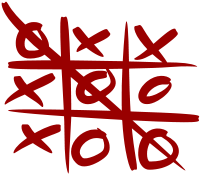
\includegraphics{./images/tictactoe.png}
  \centering
  \caption{kółko i krzyżyk}
  \label{fig:ox}
\end{figure}

Przykładowa implementacja tej gry znajduje się w pliku ox.py.
Kod programu do tej gry został też szczegółowo omówiony w dalszej części tej pracy.

\subsection{Connect Four}
W grze o nazwie Connect Four celem gracza jest takie ułożenie na planszy, żeby 4 jego pionki były połączone, podobnie jak w grze kółko i krzyżk, w pionie, poziomie lub skosie.
Gracze wrzucają swoje pionki naprzemiennie od góry planszy. Poniżej na obrazku widać przykładowy zestaw do gry - pionowa plansza z otworami na górze - do wrzucania pionków.
\begin{figure}[H]
  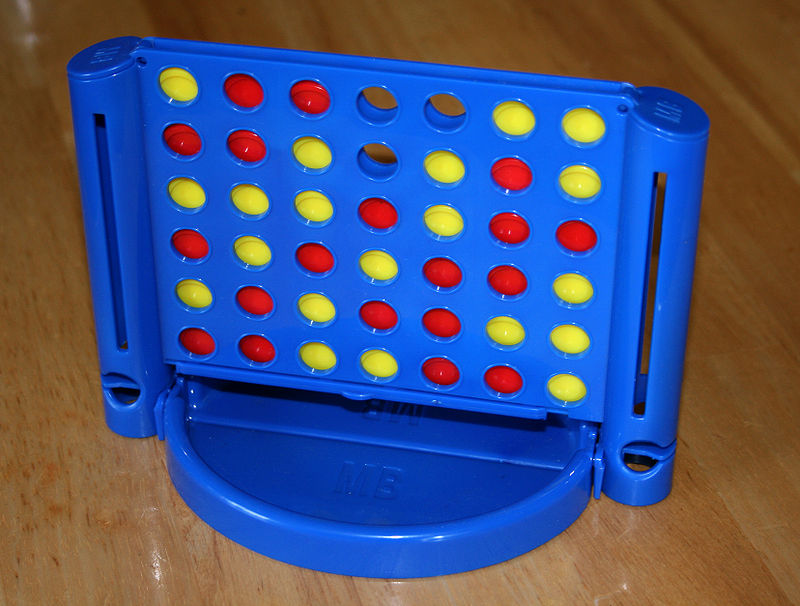
\includegraphics[scale=0.25]{./images/connect4.jpg}
  \centering
  \caption{Connect Four}
  \label{fig:c4}
\end{figure}

\subsection{Lis i Gęsi}
Tutaj zostanie omówiony podstawowy wariant gry - z jednym lisem i trzynastoma gęsiami.
Jest to prosta gra dwuosobowa. Jeden gracz zarządza Lisem, drugi gęsiami.
Gra toczy się na planszy w kształcie krzyża.
Celem Lisa jest zbicie takiej ilości gęsi by nie mogły one wygrać (zwykle 8 wystarczy).
Lis potrafi się poruszać po planszy oraz bić gęsi na takich samych zasadach jak w warcabach.
Celem Gęsi jest uwięzienie lisa - doprowadzenie do takiej sytuacji, że lis nie może się ruszyć ani zbić gęsi.
Gęsi w odróżnienu od lisa mogą się tylko przemieszczać na sąsiednie wolne pola.
Grę rozpoczynają gęsi.
Poniżej na obrazku widoczny jest wariant tej gry z dwoma lisami i większą ilością gęsi.
\begin{figure}[H]
  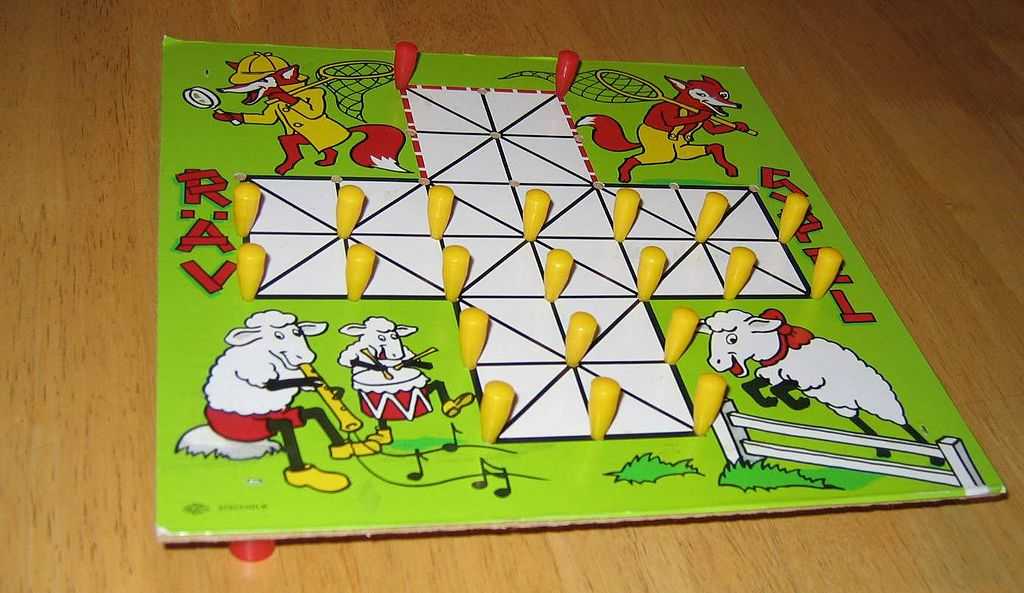
\includegraphics[scale=0.25]{./images/foxgames.jpg}
  \centering
  \caption{Fox Games}
  \label{fig:fg}
\end{figure}

Przykładowa implementacja tej gry znajduje się w pliku fox\textunderscore game.py

\subsection{Reversi}
Kolejną i ostatnią grą implementowaną na potrzeby tej pracy jest gra o nazwie reversi.
Gra odbywa się na planszy 8x8.
W grze tej jest dwóch graczy wykonujących swoje ruchy naprzemiennie.
Gracz zaczynający gra pionkami czarnymi, drugi gracz gra pionkami białymi.
Jeżeli któryś z graczy nie może wykonać poprawnego ruchu wtedy traci turę.
Gra kończy się gdy żaden z graczy nie może wykonać poprawnego ruchu.
Jeśli gracz chce wygrać powinien na zakończeniu gry mieć więcej pionków w swoim kolorze, niż przeciwnik w jego kolorze.

Teraz zostanie omówiony prawidłowy sposób wykonywania tury.
Jedyny ruch jaki można w tej grze wykonywać to dokładanie pionka.
Dokładanie pionka może odbywać się tylko w taki sposób, że tworzy linię (poziomą, pionową lub ukośną) z innym swoim pionkiem na początku (na drugim końcu lini), a pionkiem/ami przeciwnika pomiędzy (pomiędzy początkiem a pionkiem dołożonym mogą i muszą znajdować się tylko pionki przeciwnika).
Pionki przeciwnika znajdujące się na tej lini zmieniają kolor na kolor pionków gracza dokładającego.
W oczywisty sposób jednym ruchem można utworzyć więcej niż jedną taką linię - co bywa korzystne.
Poniżej znajduje się początkowe ustawienie planszy do gry w reversi.
\begin{figure}[H]
  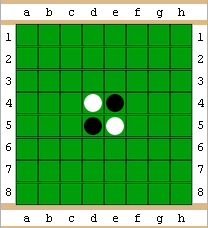
\includegraphics{./images/reversi.png}
  \centering
  \caption{Reversi}
  \label{fig:reversi}
\end{figure}

Przykładowa implementacja tej gry znajduje się w pliku reversi.py


\section{Omówienie szablonu gier planszowych}
Swoją pracę z omawianą biblioteką powinno się zacząć od zrozumienia pliku game\textunderscore template.py.
Na wstępie warto powiedzieć, że prawidłowe korzystanie z tego pliku polega na skopiowaniu go i poprawnym wyedytowaniu na potrzeby nowej gry.

\subsection{class GameTemplate}
W pliku tym znajduje się klasa GameTemplate jest to najważniejsza część tego pliku.
Jak można zauważyć klasa ta zawiera wiele metod - nazwy tych metod nie powinny być zmieniane, ponieważ agent\textunderscore module.py korzysta z nich w swoich funkcjach.
Klasa ta to abstrakcyjny model gry planszowej - zawierający wszystkie niezbędne funkcje - które powinno się zaimplementować.

\subsection{Przykładowe AI}
W tym samym pliku, poniżej wcześniej wspomnianej klasy - można znaleźć klasę NPCPlayer. Ten przykład jest bardzo prosty - jest to zwykły agent grający losowo.
W tym miejscu warto wspomnieć, że nasz moduł do agentów wykorzystuje pole player\textunderscore id - powinien być to unikatowy id dla agenta - niekoniecznie to musi być, jak w przykładzie, jego pionek.
Niemniej jednak na potrzeby funkcji z agenta to pole powinno być zapewnione.

Na końcu tego pliku widać dwie linijki kodu, które odpowiadają za inicjalizacje oraz uruchomienie gry.
\section{Propozycja implementowania gier planszowych}
Dla ułatwienia pisania programu oraz szybkiego zapoznania się z biblioteką warto omówić rutynowe czynności, które występują przy pracy z omawianą biblioteką.
Poniżej omówione są dwie zawsze występujące, rutynowe, czynności.
\subsection{Tworzenie gry planszowej}
Tworzenie gry planszowej przy pomocy tej biblioteki sprowadza się do:
\begin{itemize}
  \item Zmiany nazwy klasy GameTemplate na nazwę gry
  \item implementacji logiki gry w metodach tej klasy (zgodnie z komentarzami)
  \item implementacji interfejsu graficznego gry
  \item tetowania programu
\end{itemize}

\subsection{Tworzenie Agenta}
Tworzenie agenta w abstrakcyjnym ujęciu sprowadza sie do:
\begin{itemize}
  \item zmiany nazwy klasy agenta z pliku game\textunderscore template.py
  \item zapisanie logiki agenta w metodzie make\textunderscore move
\end{itemize}

\section{Opis agent\textunderscore module.py}
Plik agent\textunderscore module.py to tytułowy moduł, który ma ułatwiać pisanie sztucznej inteligencji do gier planszowych.
Warte omówienia (ze względu na użycie) są trzy klasy, które się tutaj znajdują:
\begin{itemize}
  \item GameBoard
  \item AgentAI
  \item HumanPlayer
\end{itemize}

\subsection{Klasa GameBoard}
Klasa GameBoard zawiera metody takie jak:
\begin{itemize}
  \item is\textunderscore on\textunderscore board - zwraca prawdę jeżeli dane współrzędne leżą na planszy - fałsz w przeciwnym wypadku.
  \item count\textunderscore symbol - zwraca liczbę wystąpienia znaku na planszy.
  \item is\textunderscore unoccupied - odpowiada na pytanie czy dane pole jest zajęte.
  \item is\textunderscore occupied - logiczna negacja poprzedniej metody.
  \item print\textunderscore board - funkcja do wypisywania na konsoli planszy
\end{itemize}
Sposoby użycia tej klasy są dobrze widoczne w dołączonych przykładowych grach.

\subsection{Klasa AgentAI}
Klasa AgentAI zawiera pola i metody - poniżej ważniejsze z nich.
Ważniejsze pola uzywane w funkcji init:
\begin{itemize}
  \item player\textunderscore id - unikatowe id gracza - służy do jego identyfikacji
  \item game\textunderscore heuristic - funkcja oceniająca grę - domyślna heurystyka symuluje losowe rozgrywki i na tej podstawie ocenia.
  \item max\textunderscore depth - maksymalna głębokość budowangeo drzewa dla funkcji takich jak minimax etc.
  \item number\textunderscore simulations - liczba symulacji dla funkcji takich jak mcts etc.
\end{itemize}

Ważniejsze metody używane w klasie agenta:
\begin{itemize}
  \item minimax\textunderscore move - funkcja zwraca ruch wybrany metodą MiniMax.
  \item random\textunderscore move - funkcja zwraca losowy ruch.
  \item alpha\textunderscore beta\textunderscore move - funkcja zwraca ruch wybrany algorytmem Alpha-Beta.
  \item mcts\textunderscore move - funkcja zwraca ruch wybrany przez algorytm Monte Carlo Tree Search.
\end{itemize}
Przykłady użycia również widoczne są w przykładowych grach np. fox\textunderscore game.py

\subsection{Klasa HumanPlayer}
Klasa HumanPlayer została zaimplementowana jako pomoc przy debugowaniu.
Jej celem jest zapewnienie minimalnej wizualizacji możliwych ruchów oraz możliwość wybrania go przez człowieka.
Klasy ta dziedziczy po AgentAI, a co więcej jest używana tak jak inni gracze w przykładowych programach.
Dla przykładu znaczy to, że aby zagrać w grę kółko i krzyży wystarczy w pliku ox.py linię:
\lstinputlisting[firstline=95,lastline=95,firstnumber=95]{../ox.py}
zamienić na:
\lstinputlisting[firstnumber=95]{humanplayer}
uprzednio importując z tego modułu klasę HumanPlayer.

\section{Omówienie kodu do gry w kółko i krzyżyk}
Na potrzeby omówienia tej pracy wybrano grę w kółko i krzyżyk.
Sama gra nie jest w żaden sposób interesująca.
Grę tą wybrano jedynie ze względu na prostotę logiki oraz zwięzłość kodu - możliwego do umieszczenia w tej pracy.
\subsection{Kod gry kółko i krzyżyk}
\lstinputlisting{../ox.py}
\subsection{Wytłumaczenie powyższego kodu}
Na początku widać klasę OX. Jest to klasa GameTemplate ze zmienioną nazwą.
Kolejno w liniach 4-9 widać inicjalizację klasy (konstruktor):
\lstinputlisting[firstline=4,lastline=9,firstnumber=4]{../ox.py}
Warto zwrócić uwagę, że na samym początku tworzymy pustą planszę do gry w kółko i krzyżyk.
kropki na naszej planszy oznaczają pola wolne.
Klasa GameBoard przyjmuje jako parametr plansze do gry (w dowolnym formacie).
W przypadku naszej gry jej użycie nie jest konieczne.
Sama ta klasa zapewnia najbardziej podstawowe funkcje do debugowania i wspomagające operacje na planszach typu tablica dwuwymiarowa.

Kolejna metoda klasy OX to get\textunderscore opponent
\lstinputlisting[firstline=11,lastline=15,firstnumber=11]{../ox.py}
Metoda ta ma na celu podanie przeciwnika dla podanego w parametrze gracza.
Jest to funkcja z której korzystają algorytmy takie jak alpha-beta, minimax - stąd potrzeba jej implementacji.

Dalej można znaleźć metody dwie kolejne metody wymagane przez bibliotekę:
\lstinputlisting[firstline=17,lastline=26,firstnumber=11]{../ox.py}

Pierwsza z tych funkcji get\textunderscore allowed\textunderscore moves powinna zwracać wszystkie możliwe ruchy dla danego gracza.
Format odpowiedzi to powinna być tablica ruchów właśiwie w dowolnym formacie, który jest rozumiany przez funkcję apply\textunderscore move.
W naszym wypadku gracz nie ma znaczenia, ponieważ możliwe ruchy to wolne pola na planszy (i nie zależy to od gracza).
Funkcja ta przyjmuje gracza jako argument tylko dla wymagań biblioteki.
Obydwie te funkcje są potrzebne do poprawnego działania algorytmów przeszukiwania.

Ostatnie dwie ważne funkcje to is\textunderscore winner oraz game\textunderscore end.
Pierwsza z nich odpowiada czy gracz podany jako argument jest zwycięzcą gry, druga odpowiada na pytanie czy gra jest zakończona.
Podobnie jak wyżej te funkcje są potrzebne dla wyżej wymienionych algorytmów i implementują logikę właściwą dla konkretnej gry.

Pozostała część kodu to funkcjonalności potrzebne do działania gry, stworzone w sposób opisana w poprzednim punkcie tego rozdziału.

\section{Propozycje dalszego rozwoju biblioteki}
Sam temat pracy jest bardzo rozległy.
Praca zaś nie pokrywa w całości tematu pracy - dlatego też zamieszczam tutaj propozycje dalszego rozwoju:
\begin{itemize}
  \item Dodanie innych prostych algorytmów (A*, DFS, BFS (wykorzystywane na kursie z AI))
  \item Przemyślenia wsparcia dla sieci neuronowych i deep learningu.
  \item Ze względu na to, że sam python działa stosunkowo wolno, a pisane programy na kursie sztucznej inteligencji są również pisane w języku C++ - stworzenie wersji blioteki w C/C++
  \item Dodanie testów automatycznych.
\end{itemize}

\chapter{Zakończenie}

Jak widać, praca nie wyczerpuje w pełni, szerokiego zagadnienia - jakim są algorytmy do gier planszowych.
Praca ta implementuje funkcjonalności, które na poziomie projektowania okazały się najbardziej znaczące.
Niemniej jednak aktualna praca pozwala na wykorzystywanie jej w wielu prostszych grach, a wymuszona architekura ma pomóc pozbyć się niepotrzebnych, powtarzalnych problemów związanych z projektowaniem kodu w grach planszowych.

%%%%% BIBLIOGRAFIA

%\begin{thebibliography}{1}
%\bibitem{example} \ldots
%\end{thebibliography}

\end{document}
